% !TeX spellcheck = en_GB_oxendict
%%%%%%%%%%%%%%%%%%%%%%%%%%%%%%%%%%% ESTADO DEL ARTE / STATE OF THE ART CHAPTER %%%%%%%%%%%%%%%%%%%%%%%%%%%%%%%%%

\chapter{Related work}
\label{cha:related-work}

\section{An introduction to the RL problem}
\label{sec:intro-rl}

\subsection{Formalizing RL}
\label{sec:form-intro-rl}
As Sutton and Barto define in \cite{intro_rl}, RL is basically learning what to do, mapping situations to actions in order to maximize a numerical reward signal. Usually, the learner is not told what to do, but instead must discover and perform the actions that get the most rewards. The RL problem usually has two main components:

\begin{itemize}
	\item \textbf{Environment}: A simulated or real world that takes actions as input and produces rewards subsequently as an output.
	\item \textbf{Agent} (the learner): which goal is to maximize the reward from the environment
\end{itemize}

The environment can be formally modeled as a Markov Decision Process (MDP). An MDP basically is a memory-less random process that is modeled by the tuple $\langle \mathcal{S,A,P,R},\gamma \rangle$, where $\mathcal{S}$ is a finite set of states where the agent can land, $\mathcal{A}$ is a finite set of actions the agent can perform, $\mathcal{P}$ is the matrix that models the transition probabilities of changing from state s to s' given an action $\mathcal{a}$ in the case of MDPs (there are cases such as Markov Reward Processes where the agent is subject to the transition probabilities and does not have autonomy or actions), $\mathcal{R}$ is the reward function that models, for a given state s and action a, the numerical reward signal that the environment will produce. It is important to not confuse the set observations from the states $\mathcal{O}$ with the set of states $\mathcal{S}$. For a MDP, the agent has total awareness of the states, and can obtain every bit of information from it. When this does not happen (i.e. a robot that has visual sensors that point only forward, and not in all possible directions), we say that the agent is in a partially observable Markov decision process (POMDP) and here $\mathcal{O} \neq \mathcal{S}$, meaning that an observation is not the same as the state. At the moment, we are dealing with MDPs, so we assume that $\mathcal{O} = \mathcal{S}$.

\begin{figure}[!h]
	\centering
	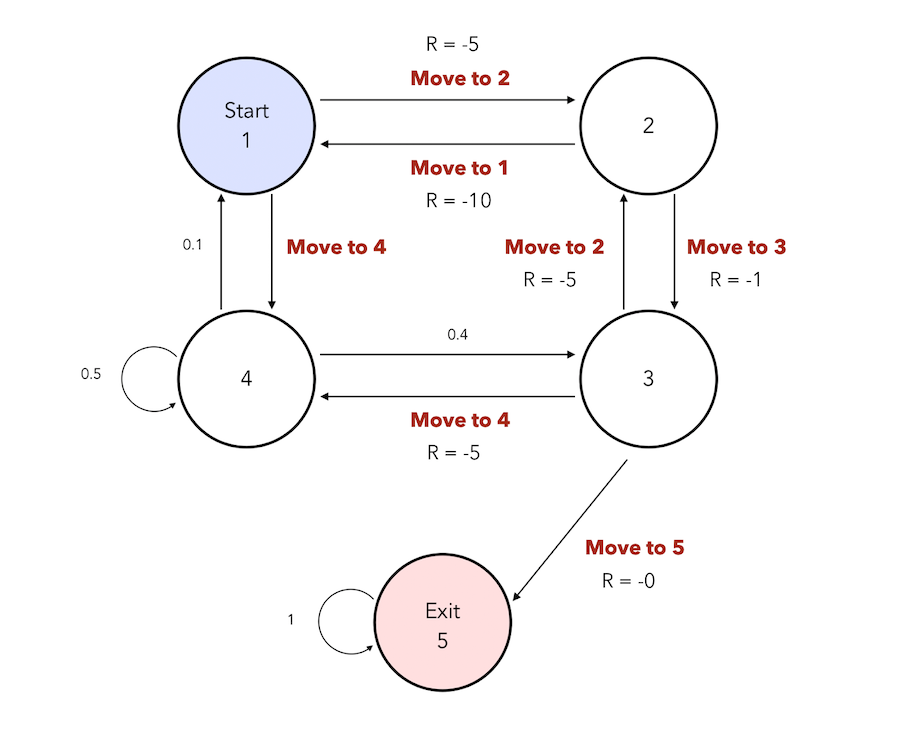
\includegraphics[width=0.8\linewidth]{figures/mdp.png}
	\caption{ (From \cite{markovdecisionprocessgithub}) Markov Decision Process with 5 states as the circles, actions are modeled with the red letters over the arrows, that represent the transition between states. When a transition is performed, a reward is returned (letter R), and a new state is achieved. We can see that there might be transitions where we cannot take an action, and we are subject to the transition probabilities (the dynamics) of the MDP.}
	\label{fig:mdp}
\end{figure} 

As we can see, the process always follows the same pattern. If we define $\mathcal{H}_t$ as the history over the MDP, we could formalize a trajectory as in equation \ref{eq:mdp_trajectory}.

\begin{equation} \label{eq:mdp_trajectory}
	\mathcal{H}_t = s_1, a_1, r_2, s_2, a_2, r_3 ... s_{t-1}, a_{t-1}, r_t, s_t
\end{equation}

Given this sequentiality in the decision making, the objective is to map this sequence of pairs state,actions (the history) to future actions that maximize the expected reward. This approach is not always useful, since in markovian processes, the current state $s_t$, is a function of the history $\mathcal{H}_t$. A markovian state uses the maxima: "\textit{the future is independent of the past, given the present}", meaning that the current state $s_t$ is a sufficient statistic of what happened in the past and it conditions what may happen next. This is formally defined in equation \ref{past_ind_fut}, where $\mathbb{P}$ represents the probability and $|$ represents the condition of a probability distribution.

\begin{equation} \label{past_ind_fut}
	\mathbb{P}[S_{t+1} | S_t] = \mathbb{P}[S_{t+1} | S_1, ..., S_t]
\end{equation}

The agent has three major components:
\begin{itemize}
	\item \textbf{Policy}: How the agent models the picked actions given a state. It may be deterministic or stochastic, and it is usually referred as $\pi$ in the notation. For example, if the policy is deterministic then we can define a mapping, such as $\pi(s)=a$, but if the policy is stochastic, then it can be defined as a probability distribution, such as $\pi(a|s) = \mathbb{P}[A=a|S=s]$.
	\item \textbf{Value Function}: A function that models how good a state is. It models a prediction of the expected future reward. Our actions usually will be influenced by how good an outcome will be by selecting an action a, given a state s. The value function models the delayed reward principle, that states that maybe an action that has a higher short-term reward, may lead to lower rewards in the future, while a low short-term reward may lead to states with higher rewards. In future sections we will formalize this concept, giving a mathematical and analytical explanation.
	\item \textbf{Model}: Useful information that the agent picks in order to build a model of the environment to understand what it might do next. This modelling consists in estimate two already known elements: the transition probability matrix $\mathcal{P}$ and the reward function $\mathcal{R}$ from the environment. Estimations are modelled by:
	\begin{enumerate}
		\item Transition probability estimation: $\mathcal{P}_{s s'}^a = \mathbb{P}[\mathcal{S'} = s' | \mathcal{S} = s, \mathcal{A} = a]$ 
		\item Reward function estimation: $\mathcal{R}_{s}^a = \mathbb{E}[\mathcal{R} | \mathcal{S} = s, \mathcal{A} = a]$ 
	\end{enumerate}
\end{itemize}

Usually, there are two types of environment modelling: model-based and model-free. In model-free RL, the agent ignores the environment's model, since it does not need to understand how the dynamics work. Instead, it uses observations and reward to build a value function and a policy that maximizes the reward. Model-based tries to make the estimations of the environment dynamics, and use them to plan and execute policies that maximize the reward. For this work, we will mainly focus on the model-free approach.

Finally, agent categorization is an important part in the RL framework. There are two principal categories (although with recent advancements, new categories have appear in the RL scene): value-based agents and policy-based agents. We will delve into this in the following sections, but we will give a brief introduction here. Value-based methods estimate the value of states in the environment and create a function that is used by the policy in order to perform actions. If only states are taken into account to provide this value estimation given a policy $\pi$, then the notation used will be $V_{\pi}(s)$. If the information to provide a value depends on both states and actions, then, we will refer to them either by ${Q}_{\pi}(s,a)$ or ${q}_{\pi}(s,a)$. On the other hand, policy-based agents only make use of policy optimization to maximize rewards, without using the value function. This two approaches can be mixed up in a symbiotic approach, using the policy and the value function to maximize the returns. This approach is usually called actor-critic methods, where the actor is the policy and the critic is the value function.

\subsection{Value-based RL}
\label{sec:val-based-rl}
In model-free RL, we do not have any clue of the environment's dynamics. Still, proper choices need to be done in order to maximize rewards. A value function estimates how good an state is, not only for the short-term, but also for the long term. This value function is also conditioned on a given policy $\pi$, so we will define the value function as in equation \ref{eq:state_value}, where we define the episodes of experience following a policy as $S_1, A_1, R_2, ..., S_k \sim \pi$ and the returns $G_t = R_{t+1} + \gamma R_{t+2} + \gamma^2 R_{t+3} ... + \gamma^{T-1}R_{t-1}$.

\begin{equation} \label{eq:state_value}
	V_{\pi}(s) = \mathbb{E}_{\pi}[G_t | S_t = s]
\end{equation}

For various purposes, the state information may not be sufficient to estimate the value of a state itself, so the action must be part of the value associated. Formally, it is described as in equation \ref{eq:action_value} and this kind of values are formally known as action values.

\begin{equation} \label{eq:action_value}
	q_{\pi}(s,a) = \mathbb{E}_{\pi}[R_{t+1} + \gamma q_{\pi}(S_{t+1},A_{t+1}) | S_t=s , A_t=a]
\end{equation}

Usually, in model-free reinforcement learning ${Q}$-values are common approach, since with the state values, the environment dynamics $\mathcal{P}$ should be at least known or estimated. This is why in following sections, the formulation will be more focused on ${Q}$-values. Section \ref{app:on-policy-control} expands on this matter.

There are several approaches that make use of the value function definition to make estimations about it. In this section we will briefly go over Temporal Difference Learning: TD(0) and a two special cases: Deep Q-Networks (DQN) and Double Deep Q-Networks (DDQN). Again, if deeper insights are needed, we encourage the reader to take a look at section \ref{app:classic_rl} where we explain in depth several important aspects of methods like Monte Carlo learning or TD learning. Our main focus will be in the value function approximators, since this is when deep learning made its appearance in the RL framework.

\subsubsection{Value function approximation} 
\label{sec:val-fun_approx}

Environments in RL may end up being quite complex. This complexity usually comes from the number of possible states of our environment. For example, a robot walking down a street finds itself constantly in new states, as the observation of the environment changes constantly (i.e people coming by, cars running down the street... etc). Creating a table that models such a complex space may be infeasible, but we can use and optimize a high parameterized function to approximate the optimal value function, and here is where deep neural networks make their appearance. Formally, the goal of the optimization is described in equations \ref{eq:value_aprox} and \ref{eq:q_value_aprox}, where \textbf{w} is a vector that holds the weights (or parameters) from the function approximator.

\begin{equation}\label{eq:value_aprox}
	\hat{V}(s,w) \approx V_{\pi}(s)
\end{equation}

\begin{equation}\label{eq:q_value_aprox}
	\hat{q}(s,a,w) \approx q_{\pi}(s,a)
\end{equation}

In this section we are going to focus on the action value function $\hat{q}(s,a,w)$. This function approximator could be defined as the combination of the input features $\phi$ by the weights (eq. \ref{eq:comb_qval}).

\begin{equation} \label{eq:comb_qval}
	\hat{q}(s,a,w) = \phi(S,A)^T w = \sum_{j=1}^{n}\phi_{j}(S,A) w_j
\end{equation}

The objective of Value Function Approximation is similar to a supervised learning scenario. In equation \ref{eq:sgd_objective_function} it is defined to minimise the Mean Squared Error (MSE) of the difference between the objective function $q_{\pi}(s,a)$ and the approximation $\hat{q}(s,a,w)$. This optimisation is done via Stochastic Gradient Descent (SGD) (equation \ref{eq:sgd_opt}) where we derive the MSE with respect to the set of parameters w, looking for the steepest part of the curve for descending it in order to minimize the error. Since we do not have the objective function $q_{\pi}(s,a)$, we must adjust our parameters to the estimations we collect as we explore the state space.

\begin{equation} \label{eq:sgd_objective_function}
	\mathcal{J}(w) = \mathbb{E}_{\pi}[(q_{\pi}(S,A) - \hat{q}(s,a,w))^2 ]
\end{equation}

\begin{equation} \label{eq:sgd_opt}
	-\frac{1}{2} \nabla_{w} \mathcal{J}(w) = (q_{\pi}(S,A) - \hat{q}(s,a,w)) \nabla_{w}\hat{q}(s,a,w)
\end{equation}

This approach can be applied to TD learning for example. In the case of TD(0) (equation \ref{eq:value_approx_td0}), the adjustments for the weights of the function approximation $\Delta_{w}$ would be done using the difference of the information we already know $\hat{q}(s_{t},a_{t},w))$ and the new information that we have acquired with the new transition $R + \gamma \hat{q}(s_{t+1},a_{t+1},w)$. The same is done for TD($\lambda$) in equation \ref{eq:value_approx_tdlambda}.

\begin{equation} \label{eq:value_approx_td0}
	\Delta_{w} = (R + \gamma \hat{q}(s_{t+1},a_{t+1},w) - \hat{q}(s_{t},a_{t},w)) \nabla_{w}\hat{q}(s_{t+1},a_{t+1},w)
\end{equation}

\begin{equation} \label{eq:value_approx_tdlambda}
	\Delta_{w} = (q_{t}^{\lambda} + \gamma \hat{q}(s_{t+1},a_{t+1},w) - \hat{q}(s_{t},a_{t},w)) \nabla_{w}\hat{q}(s_{t+1},a_{t+1},w)
\end{equation}

One of the biggest success in the value function approximation paradigm is Deep Q-Networks (DQN) \cite{mnih2013playing} that uses Q-Networks to estimate the value function using neural network. This algorithm first produces experiences and stores them into the experience buffer $\mathcal{D} = \{(s_i, a_i, r_i, s_{i+1}, d_i)\}_{i=1}^N$, where N is the size of the buffer. Then, with an off-policy Q-leaning approach, a loss function (equation \ref{eq:dqn_loss}) is proposed. The main goal is to minimize the MSE, and, as it does, it learns a value function that produces the ${Q}$-values for each possible action.

\begin{equation} \label{eq:dqn_loss}
	\mathcal{L}_w = \mathbb{E}_{\mathcal{D} \sim s, a, r, s'} \left[ \left( r + \gamma \max_{a'} Q(s', a'; w^-) - Q(s, a; w) \right)^2 \right]
\end{equation}

\noindent where:
\begin{itemize}
	\item $Q(s, a; w)$: represents the neural network with the updated weights.
	\item $Q'(s', a'; w^-)$: represents the frozen neural network with the previous weights.
\end{itemize}

The main intuition behind this loss function resides in the offline network $Q(s', a'; w^-)$ as a force that tries to maximize reward at each possible future state s' with the weights of previous iterations $w^-$, and the online network $Q(s, a; w)$ that tries to minimize the gap of its predictions, but for the current state s. This makes the online network to update its predictions towards what the offline network is maximizing, giving a good estimate of the Q values for a given present state s and an action a. Years later, Double Deep Q-Networks (DDQN) \cite{vanhasselt2015deep} made a few updates upon DQN, achieving ever better results. The goal is to minimize the loss function presented in equation \ref{eq:ddqn_loss} 

\begin{equation} \label{eq:ddqn_loss}
	\mathcal{L}_w =  \mathbb{E}_{\mathcal{D} \sim s, a, r, s'} \left[ \left( r + \gamma Q(s', \operatorname*{argmax}_{a'} Q(s', a'; w); w^-) - Q(s, a; w) \right)^2 \right]
\end{equation}

The motivation behind this update mainly reside in the fact that DQN overestimates the Q-values, which bias the agent into thinking that some state are more valuable that what they really are. This is because in the DQN loss, the action selection is done by maximizing the estimates of the target network, but, since we are trying to evaluate how good the online network is doing, it makes more sense that the action evaluated by the target network is selected by the online network, which gives us a better idea of how the agent is performing since the online network is the one used on the behaviour policy.

\subsection{Policy-based RL}
\label{sec:pol-grad-ac}
In the value based methods, the policy usually is deterministic. In section \ref{app:on_policy_control}, we go deeper in exploring greedy and $\epsilon$-greedy policies as a mapping from state/action value functions to actions, but the main important take, is that deterministic policies are not always enough for some complex environments. We can make use of parameterization in order to make our agent more capable of dealing with harder problems expanding the representation capabilities for decision making. A good policy usually is the one that maximizes the reward in each time-step, so we must always look in the direction that provides greater expected rewards using action selection. 

\subsubsection{Policy Gradient Theorem}
\label{sec:pol-grad-theorem}
The parametrized policy is defined as in equation \ref{eq:param_policy}. Where $\theta$ is the parameter vector of our function approximator (i.e. a neural network).
\begin{equation} \label{eq:param_policy}
	\pi(a|s, \theta) = \mathbb{P}[a|s, \theta]
\end{equation}

These parameters must converge to a solution where our policy maximizes the rewards, taking actions that consequently do so. The policy gradient theorem states that in order to obtain the optimal policy $\pi^*(a|s, \theta)$ that maximizes the rewards, we must compute the gradient defined in equation \ref{eq:policy_gradient_theorem}
\begin{equation} \label{eq:policy_gradient_theorem}
	\nabla_{\theta}\mathcal{J}(\theta) = \mathbb{E}[\nabla_{\theta} log (\pi_{\theta}(s,a)) {Q}^{\pi_{\theta}}(s,a)]
\end{equation}

Where the term $\nabla_{\theta} log (\pi_{\theta}(s,a))$ gives us a likelihood estimation of how much does the agent want to be in the same state and action pair. If the reward is big, we want that gradient to be big, and follow that direction, using Stochastic Gradient Ascend (SGA). On the other hand, the term ${Q}^{\pi_{\theta}}(s,a)$ measures how beneficial was taking the action a. It ponders the direction of the gradient we want to maximize. If we had a situation of great value, then that gradient should be explored more, hence the bigger values, but, if the gradient or the value is low, the agent should not be in that position very often, to avoid loss of potential reward.

One of the first policy gradients method is REINFORCE. It is based in the Monte Carlo learning method. Here ${Q}^{\pi_{\theta}}(s,a) = v_t$, where $v_t$ is the cumulative expected reward for time-step t. The weight updates are done as defined in equation \ref{eq:reinforce}, where t is the current time-step. For further reading, more in depth detail about different policy gradients methods such as Actor-Critic (A2C) is discussed in section \ref{sec:ac-methods}.

\begin{equation}\label{eq:reinforce}
	\Delta\theta_{t} = \alpha(\nabla_{\theta} log \pi_{\theta}(s,a)v_t)
\end{equation}

\section{Attention-based models}
\label{sec:attention}

\subsection{What is attention?}
\label{sec:whats-attention}
The attention mechanism was first introduced in \cite{bahdanau2016neural}. There, the authors explain how difficult is to make translations from different languages. The issue in particular was the alignment, meaning that the number of tokens or words in a translated sentence usually is different compared to said sentence in the original language. This presented a challenge for the network since it had to detect which parts of the original sentence produced the resulting translation at token level. For example, the word "crosswalk" in English, translates to Spanish as "paso de peatones" which is not a literal translation. Therefore, the task presented in this particular example would be to teach the network to align a single word in English to the counterpart three words in Spanish. We encourage the reader to go to section \ref{app:attention-mec} for further reading on the details of the attention mechanism.

The authors tackled this problem by using an recurrent encoder-decoder architecture using recurrent neural networks (RNNs) as presented in figure \ref{fig:alignmentattention}, extracted from \cite{understandingattentionmechanism}. The encoder is based on an Bidirectional Long-Short-Term-Memory (Bi-LSTM) network, that takes the token embeddings from the input, and process them creating the vector $h_j$, which contains all the information from the input up to time-step $j$. The decoder is another RNN network that has as input a context vector $c_i$ and maps it to a hidden state vector $s_i$ and an output vector $y_i$, where $i$ is the time-step of to the output. The context vector $c_i$ is obtained by pondering the embeddings produced by the encoder using vector $\alpha_i$. 

\begin{figure}[!h]
	\centering
	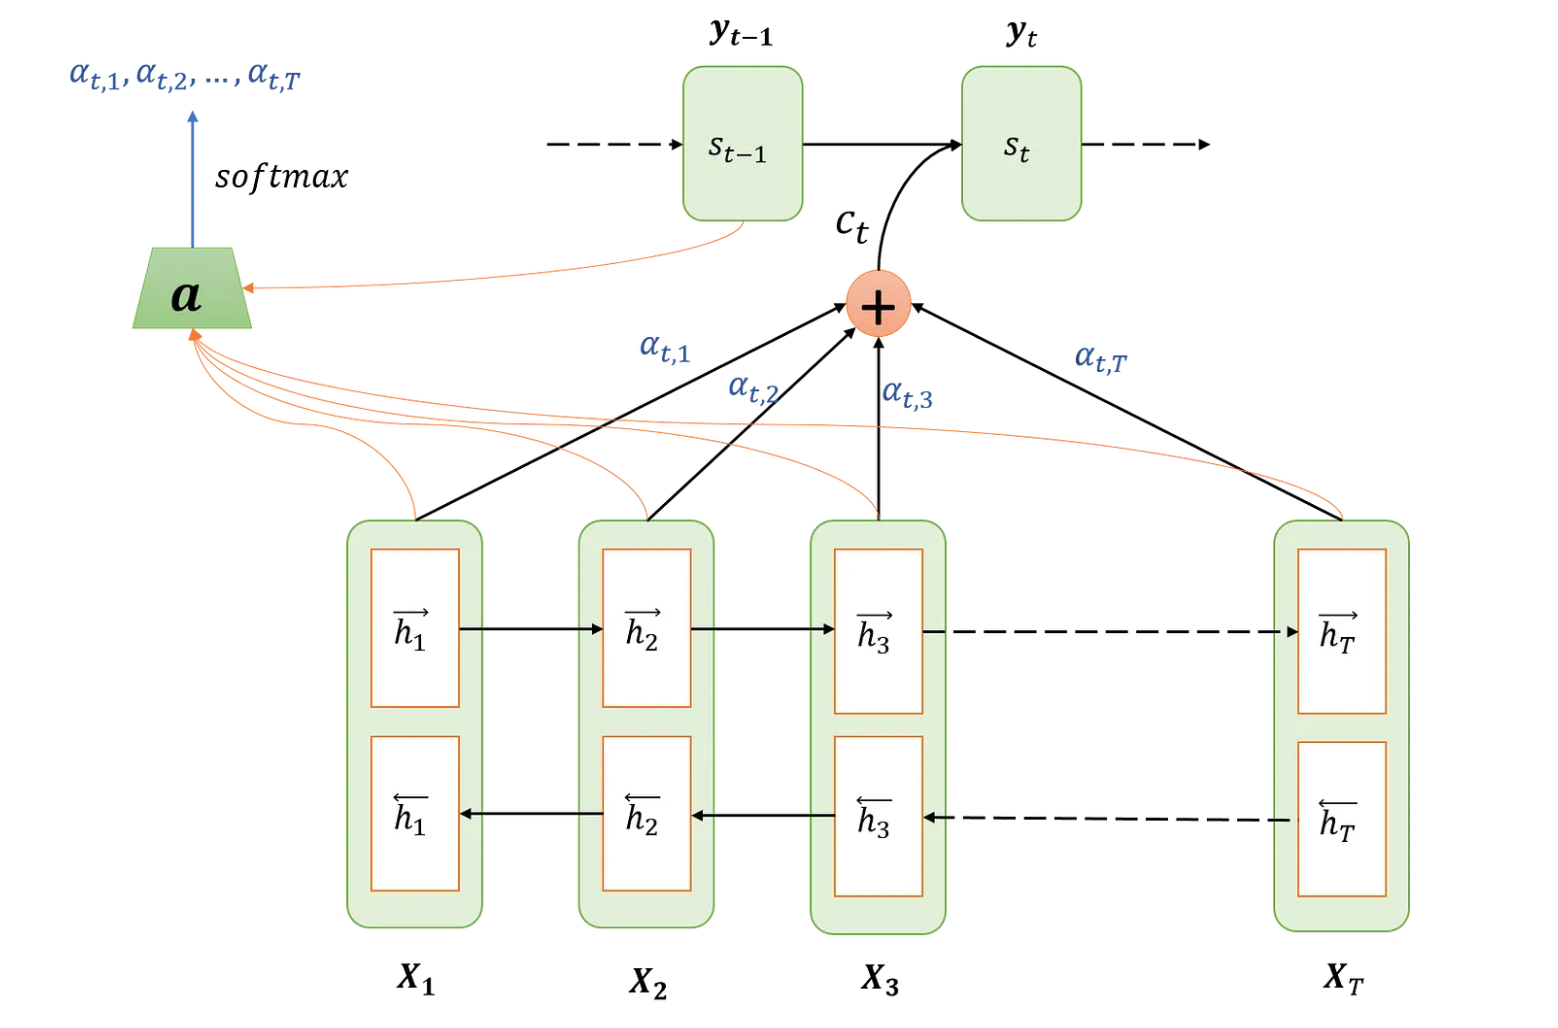
\includegraphics[width=0.7\linewidth]{figures/alignment_attention}
	\caption{Aligning inputs using the attention mechanism. First, the inputs $X_1, X_2, X_3, ... X_{\tau}$ are encoded using a bi-directional RNN, obtaining the embeddings $\protect\overrightarrow{h} , \protect\overleftarrow{h}$. This embeddings are then pondered by the product of the learnable parameters $\alpha_{i \tau}$ for each input, creating the context vector $c_t$. Finally, $c_t$ is fed into the decoder, updating the hidden state $s_t$ and producing the output $y_t$.}
	\label{fig:alignmentattention}
\end{figure}


\subsection{The Transformer Architecture}
\label{sec:transformer}

The architecture introduced in section \ref{sec:whats-attention} had its limitations, especially in modelling dependencies between sections of the input text that were far apart. This was because the fixed compressed representation (the embedding) of the input of the decoder only holds information from the closest tokens, not being able to model long-range dependencies. To tackle this problem the Transformer architecture  \cite{vaswani2023attention} introduced self-attention, where the whole sequence is processed at once and the dependencies are computed altogether, instead of processing the inputs one per time-step. Self-attention is defined as in equation \ref{eq:attn_eq}, where Q, K, and V represent the query, key, and value matrices, respectively, $d_k$ represents the dimensionality of the keys and queries, $\sigma$ represents the soft-max function applied along the rows of the matrix resulting from the dot product of Q and $K^T$. This creates a vector of weights that ponder the importance of each element of the input with respect to the rest of the elements, describing how relevant are for the model. Finally, this weights are multiplied element-wise with the value matrix V to compute the final attention output. We can think about the query (Q) as a vector that holds information about what each token in the input is looking for, meaning, which other tokens is interested in. On the other side, the keys (K) represent the information each token from the input holds. When transforming the input onto the query-value space, vectors (embeddings) that are close will have a higher dot product result, meaning that the "energy" of their semantic relation is bigger. On the other hand, if those vectors are quite far, the dot product will be smaller, hence, the energy will be lower, meaning that those vectors are not quite related. The implications that this work had in the AI research field were huge, and it was in part, because it, revealed a new upcoming discovery for explainability in neural networks, thanks to the weights the attention matrix holds

\begin{equation} \label{eq:attn_eq}
	\text{Attention}(Q,K,V) = \text{$\sigma$}\left(\frac{QK^T}{\sqrt{d_k}}\right)V
\end{equation}

What we have explained up until now it is know as an attention "head", this means that there is only one participant looking for relevant information in a sequence, but, it is well known that having several model instances cooperating to solve a problem is always better \cite{model_emsembling_survey}. In order for the attention mechanism to look at different parts of the inputs at the same time, we need multiple instances looking at different parts and communicating between them. This is known as Multi-Head Self Attention (MHSA). When we have multiple attention heads \cite{vaswani2023attention}, we can extract a rich feature map that ponders the important of different parts of information from the input. Because multiple heads can focus on different parts of the input, our attention maps will be quite diverse, preventing over-fitting. This approach also takes advantage of distributed computation, because computing the self-attention for each attention head can be done in parallel, making it efficient in time. Figure \ref{fig:multihead_attn} provides a diagram that explains the very same concept discussed in this section.

\begin{figure}[!h]
	\centering
	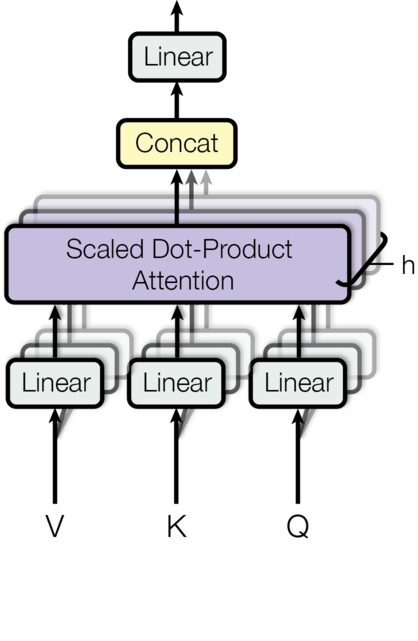
\includegraphics[width=0.25\linewidth]{figures/multi_head_attn.png}
	\caption{Multi-head attention. The embeddings from Q, K and V are computed and fed into the attention module. Once computed, the attention matrix is computed for each of the heads, and concatenated to then, be forwarded onto a linear layer, that computes the embedding of the attention-weighted input.}
	\label{fig:multihead_attn}
\end{figure} 

In figure \ref{fig:transformer_arch}, we can see the complete transformer architecture. First we can the encoder, that uses attention to generate the embeddings of the sequence, where in each time step, the attention heads will focus in different parts of the input. Then, the decoder takes those embeddings and starts producing the outputs in an auto-regressive manner, taking its own outputs as input embeddings to the decoder that are mixed with the embeddings of the encoder, to provide a wider context of the whole sequence.

\begin{figure}[!h] 
	\centering
	\subfloat[Transformer architecture.]{%
		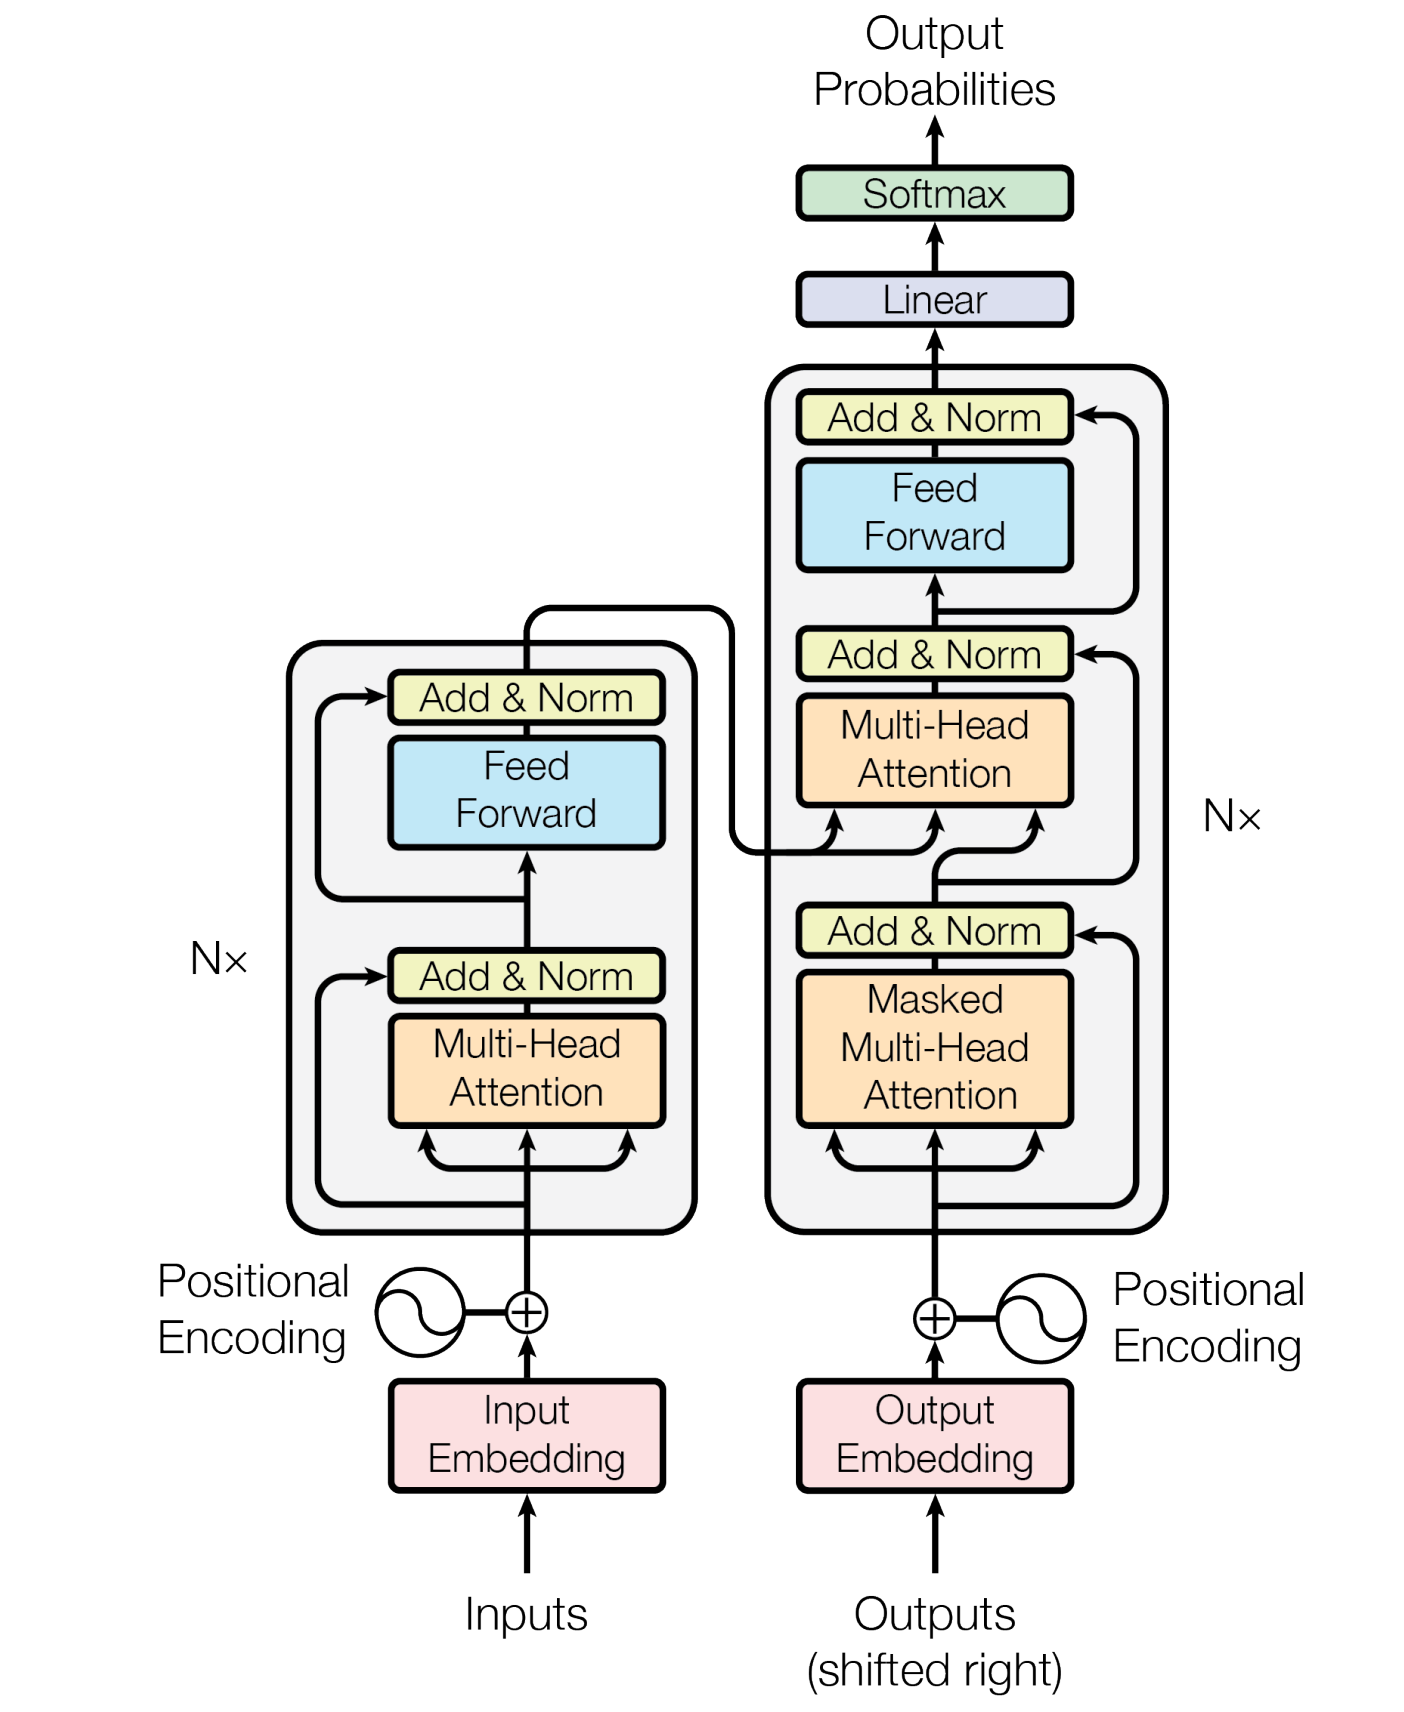
\includegraphics[width=0.5\linewidth]{figures/transformer_architecture.png}%
		\label{fig:transformer_arch}%
	}%
	\hfill%
	\subfloat[Cross-Attention weights for the translation task]{%
		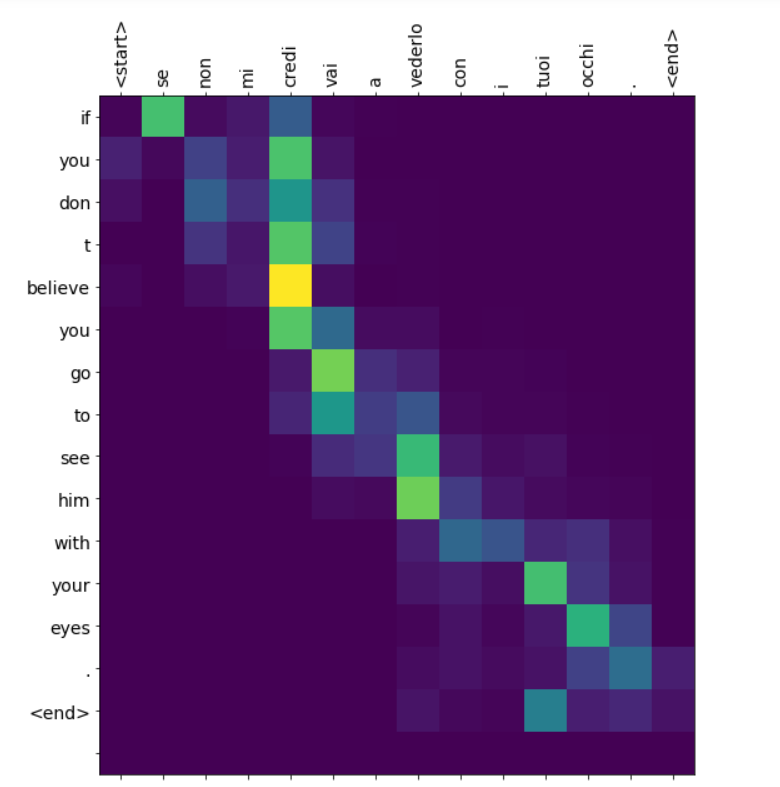
\includegraphics[width=0.5\linewidth]{figures/text_translation_attn.png}%
		\label{fig:translation_attn}%
	}%
	\caption{In figure \ref{fig:transformer_arch} (left), from \cite{vaswani2023attention}, the complete transformer architecture is presented. In figure \ref{fig:translation_attn} (right) from \cite{translationmin2023attention}, an attention matrix is presented for a sentence and its translated counter-part. The weights for each word quantify how much \textit{attention} is the model paying to the words from the original sentence in order to produce the translation to the new sentence.}
\end{figure}


Naturally, one can see the attention weights are the main piece of information that explains the output. Attention weights provide a numerical description of which parts of the input the algorithm is looking for, thus providing an approximate explanation of the output. In figure \ref{fig:translation_attn} we have an example of how a transformer performs translation between English and Portuguese, providing the correct alignments for each word. 

\subsection{Vision Transformers}
\label{sec:vis-transformers}
Self-attention is a powerful mechanism, that can be applied not only to sequences, but also to visual data. The vision transformer (ViT) \cite{vit} was one of the first models that leveraged the self-attention mechanism in order to process images. The architecture is presented in figure \ref{fig:vit_arch}, where the first thing to notice is that there is only an encoder in the architecture. This is because this model was designed for image classification, and the best approach to solve this task is to extract an embedding as a compressed representation of the original image. The input is processed by patching the image, creating different blocks that serve as input. To take context of which patch is in which position of the image, the ViT model has a learnable parameter that serves as an absolute positional embedding. Then, the attention heads will look at each of the patches separately. To do this, the ViT flattens the patches from the images and treats it as a sequence, paying attention to the features from the raw input that are more relevant. By having several attention heads looking at several patches at the same time, the model captures global dependencies between them, obtaining a rich representation of the image. After that, the attention matrix computed from each head is concatenated and forwarded into a multi-layer perceptron (MLP) that produces the embedding that the classifier will use to produce the output.

\begin{figure}[!h] 
	\centering
	\subfloat[Transformer architecture.]{%
		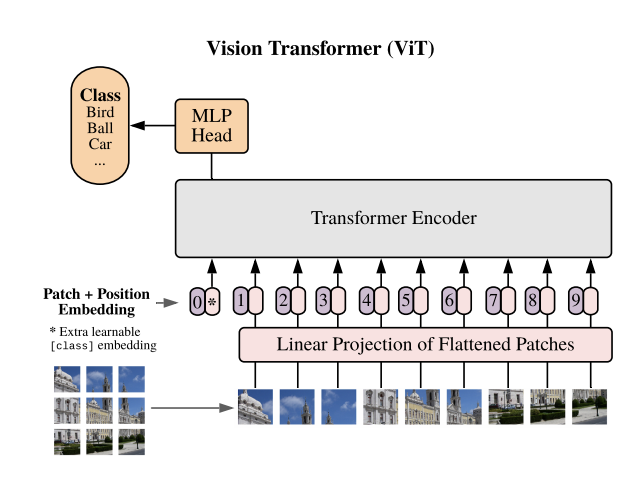
\includegraphics[width=0.5\linewidth]{figures/vision_transformer.png}%
		\label{fig:vit_arch}%
	}%
	\hfill%
	\subfloat[Attention weights for human detection task]{%
		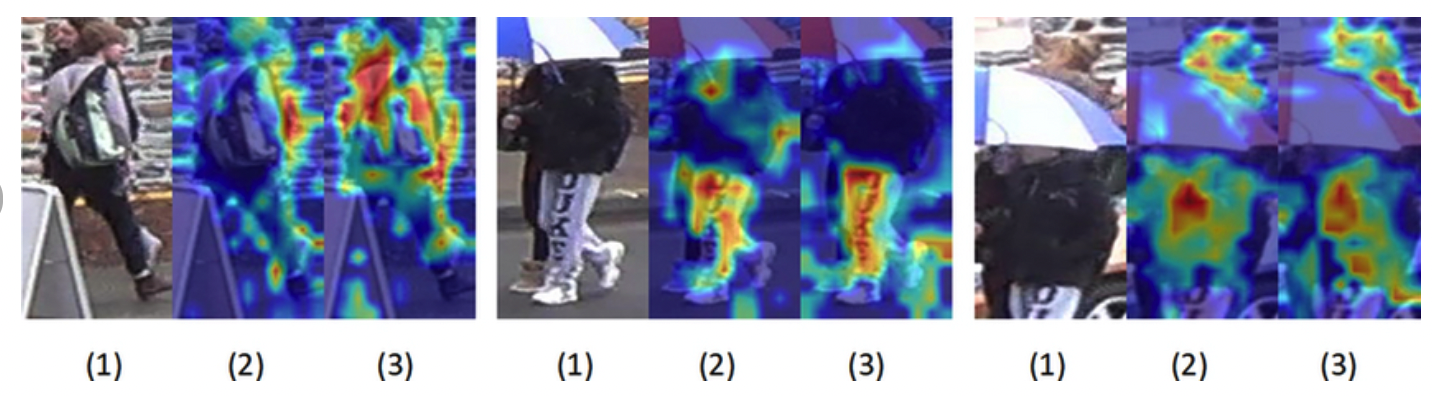
\includegraphics[width=0.5\linewidth]{figures/visual_attention_occlusion.png}%
		\label{fig:attn_maps}%
	}%
	\caption{In figure \ref{fig:transformer_arch} (left) the ViT transformer architecture is presented. In figure \ref{fig:translation_attn} (right) an attention map is presented. The model that produced the attention maps was trained to track people on a scene, and it is why, the higher attention weights (red) are put in the pixels where people is present.}
\end{figure}


\subsection{SWIN Transformer}
\label{sec:swin-transformer}
One of the main issues that the ViT model holds, is the computational cost of the self-attention module being quadratic. This means that, as images are bigger, the number of patches where the attention is performed will increase, making the input embeddings more expensive to process. To solve this, the SWIN Transformer \cite{liu2021swin} (figure \ref{fig:swin_transformer_parts}) takes an alternative approach, and uses a hierarchical architecture that resembles the CNNs. First, it divides the image in patches, as the ViT model does, but, instead of computing the attention, it adds the concept of window attention to the mix. A window will contain a set of patches, and the attention will be performed between the patches that are inside the window. This reduces the complexity of the attention operation, but at the cost of global feature extraction, since the patches inside of a window only know the existence of themselves, but not of their neighbours under a different window. To solve this, the SWIN Transformer introduces masked window shifting and patch merging. 


\begin{figure}[htbp]
	\centering
	\begin{subfigure}{0.28\textwidth}
		\centering
		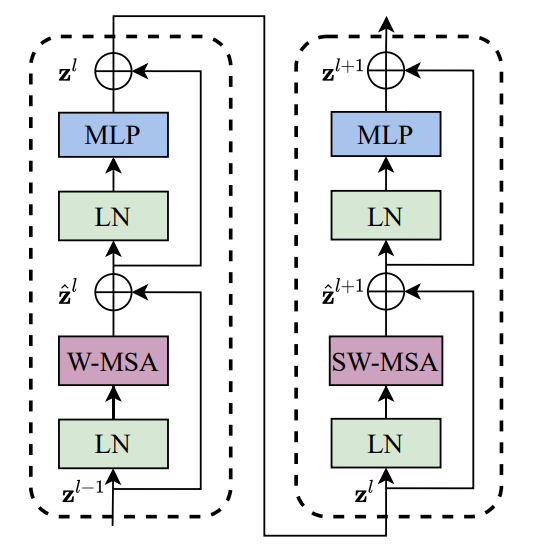
\includegraphics[width=\textwidth]{figures/swin_blocks}
		\caption{Swin Transformer block}
		\label{fig:swinblocks}
	\end{subfigure}
	\begin{subfigure}{0.7\textwidth}
		\centering
		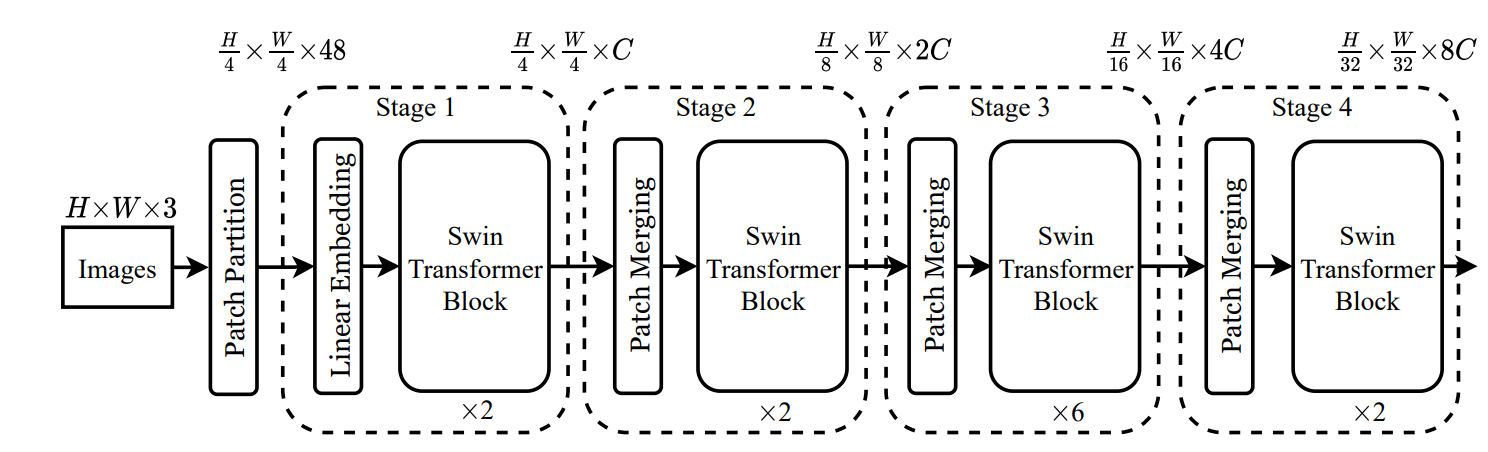
\includegraphics[width=\textwidth]{figures/swin_architecture}
		\caption{SWIN Transformer architecture}
		\label{fig:swinarchitecture}
	\end{subfigure}
	\caption{Swin Transformer architecture and its building blocks. The transformer block, figure \ref{fig:swinblocks}, has two phases. In the first one (left-most block), it performs a layer normalization, followed by a window-MSHA block that is forwarded onto a MLP with a neurons ratio of 4. In the second, it makes use of the shifted window MSHA, instead of the window-MHSA. In figure \ref{fig:swinarchitecture} we can see the whole SWIN Transformer architecture, where each of the "stages" are built upon the transformer blocks, that have as input the patch merged embeddings that are passed at each stage.}
	\label{fig:swin_transformer_parts}
\end{figure}

Masked window shifting, presented in figure \ref{fig:windowshifting} is a simple but effective procedure to broaden the spatial context of the windowed attention. The intuition is to drift the layout of the patches inside the image, providing a wider spatial context to the attention performed inside the windows. This means that the group of patches that are left out of the image (sections A, B, C) are mirrored to the symmetric part of the image, performing a \textit{"cyclic shift"}. This cyclic shift alters the spatial disposition of the elements in an image, since the parts of the top left are now in the bottom right. To handle this, they provide a mask that ensures that the shifted regions only attend to their corresponding parts. For example, the patches inside region A will only attend to patches that are only inside said, region. This ensures that the spatial information remains unaltered and no "abnormal" representations are learn as a product of this shifting. 

On the other side Patch Merging, figure \ref{fig:patchmerging}, is an operation that uses concatenation along the channel dimension to aggregate the features from the patches inside a window. This provides a hierarchical architecture, where the local features are captured in the first stages of the architecture, since the spatial dimension is bigger, and the global features are captured at the latest stages, where the spatial dimension is diminished, and all the local features are aggregated along the channel dimension. The patches are selected in a 2 by 2 grid, so the input has a shape of $W \times H \times C$, and after the patch merging, has a shape of $\frac{W}{2} \times \frac{H}{2} \times 4C$. In some type of way, this could be seen as a \textit{"convolutional transformer"}, since it quite resembles some of the hierarchical mechanisms that the CNNs have to perform feature extraction from an image. 

\begin{figure}[!h]
	\centering
	\begin{subfigure}{\textwidth}
		\centering
		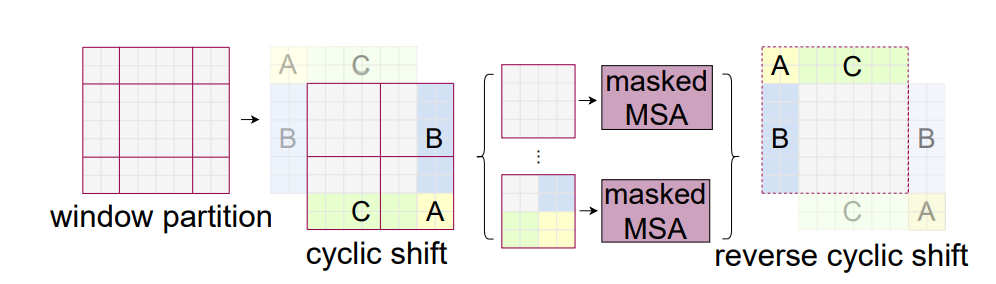
\includegraphics[width=0.8\linewidth]{figures/windowshifting}
		\caption{Window shifting and cyclic shifting module}
		\label{fig:windowshifting}
	\end{subfigure}
	\hfill
	\begin{subfigure}{\textwidth}
		\centering
		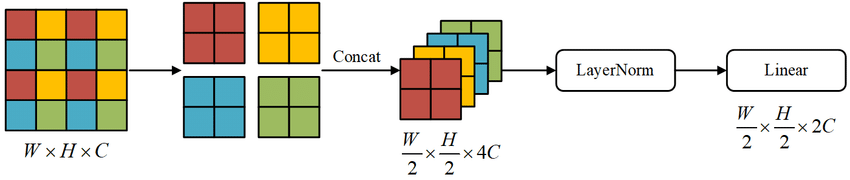
\includegraphics[width=0.9\linewidth]{figures/patch_merging}
		\caption{Patch merging module for hierarchical feature aggregation (image from\cite{swin_unet})}
		\label{fig:patchmerging}
	\end{subfigure}
	\caption{Window shifting in the SWIN Transformer architecture (figure \ref{fig:windowshifting}). From the window partition, shift to the bottom right, so the A, B, C patches are rearranged in the mirrored side of the image. Patch Merging (figure \ref{fig:patchmerging}), picks blocks of 2 by 2 patches inside a window and concatenates them along the channel dimension.}
	\label{fig:combined}
\end{figure}

\section{Explainable AI}
Explainable AI (XAI) refers to techniques and methods that make the behavior and decisions of artificial intelligence systems transparent, understandable, and interpretable to humans. It aims to clarify how AI models reach their conclusions, enhancing trust, accountability, and usability, especially in critical applications like healthcare and finance. The concept of explainable AI has been around for quite some time. In the eighties, in \cite{swartout1985explaining}, Swartout explains that the need for systems that have "cognitive" abilities to solve complex problems must come with an explanation, and developed a basic rule-system to explain the results. It is clear that, since the AI research began, researchers have always claimed the need for mechanisms and systems to explain decision making. There are some AI models that are quite good at, this, like decision trees, since is quite common to follow down the nodes and leaves (questions and conditions that the tree proposes in order to perform inter-class separability) in order to understand the decisions performed to classify a given input with a certain class, presenting a reasoning of a final decision. The issue comes when the complexity of the model increases. For example, a random forest is a set of decision trees that jointly participate in a poll to determine, the class of a given input. The set of decision trees can be huge for complex datasets, and to trace each and everyone of the decisions performed by all of the trees can be an exhaustive process. Something similar happens with deep neural networks. With the appearance of AlexNet \cite{alexNet} in the ImageNet challenge \cite{ILSVRC15}, a shift of paradigm appeared, since the following years, deeper models were presented to the challenge. Results at the time were astonishing, but with a cost, since as the network got deeper, the interpretation of the activation maps in the receptive fields of the layer was almost impossible, which led to a big concern: what is the network looking at in order to make the predictions? One thing is clear, as shown in Figure \ref{fig:explainablechart} from \cite{Turek2017}, the accuracy is higher when less explainable is the model.

\begin{figure}[!h]
	\centering
	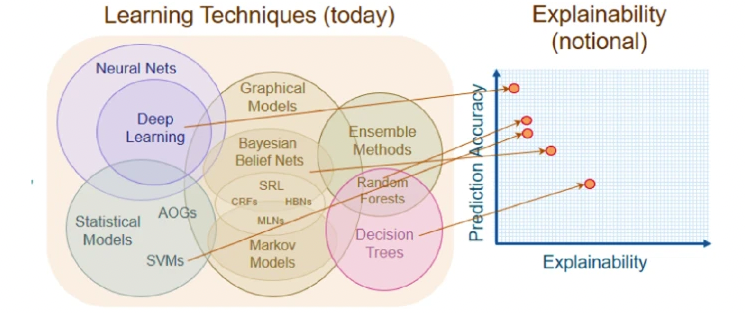
\includegraphics[width=0.7\linewidth]{figures/explainable_chart}
	\caption{Explainability of ML models against the prediction accuracy.}
	\label{fig:explainablechart}
\end{figure}

in the past decade, the field of computer vision has been involved a pursuit to make DNNs transparent and understandable. In the following sub-sections we will briefly explain the techniques that have been used in this work along with another relevant works from the XAI field.

\subsubsection{Sensitive Analysis}

In \cite{xai_survey2019, sensitivity_analysis}, sensitive Analysis (SA) is defined as a method that identifies which parts of the input are more sensitive to the network to perform the predictions. To do so, it assumes that the most relevant input features are the most sensitive for the output, and by "obstructing" pixels or sections of the image, it ponders how relevant are different sections to the predicted output. The mathematical definition behind this concept is defined in equation \ref{eq:grad_sensanalysis}, where they define all the partial derivatives for a function $f(x)$ as the sensitivity $s_{ik}$ of the network to a certain input $x_n$ with respect to all the i-th elements of the input $x_i$ and the output $y_k$.

\begin{equation}
	\label{eq:grad_sensanalysis}
	s_{ik} \bigg|_{\mathbf{x}_n} = \frac{\partial y_k}{\partial x_i} (\mathbf{x}_n)
\end{equation}

The issue that appears with SA is that it does not explain the function approximation performed by the neural network, but only quantifies the importance of the input. This may not be ideal, as we want to understand what the network gives more importance to with respect to the features of the input, not understand which parts of the network are essential to produce the output.

\subsubsection{Layer-wise Relevance Propagation}
Layer-wise Relevance Propagation (LRP) \cite{bach2015pixel} is an interpretability method used to explain the predictions of neural networks. The main idea of LRP is to propagate the prediction score $f(x)$ backwards through the network layers, assigning relevance scores $R_i$ to each neuron in the network.

There are several variations of LRP to interpret neural network predictions, but one of the most useful ones is the LRP-$\alpha\beta$, which ponders between the positive and negative contributions to the prediction, given an input. The relevance $R_i$ of each neuron $i$ is traced back layer by layer, indicating the contribution of each neuron to the final prediction. To distinguish between positive and negative contributions, LRP decomposes the term $Z_{ij} = a_i^{(l-1)} \cdot w_{ij}$, where $a_i^{(l-1)}$ is the activation of neuron $i$ and $w_{ij}$ is the weight connecting neuron $i$ to neuron $j$. The positive and negative parts are defined as $z^+_{ij} = \text{max}(0, z_{ij})$ and $z^-_{ij} = \text{min}(0, z_{ij})$. The  LRP-$\alpha\beta$ then, combines these parts to propagate the relevance from the current layer $l$ to the previous $l-1$, as defined in equation \ref{eq:lrp_alphabeta}

\begin{equation}
	\label{eq:lrp_alphabeta}
	R_i^{(l-1)} = \sum_j \left( \alpha \frac{z_{ij}^+}{\sum_{i'} z_{i'j}^+} R_j^{(l)} - \beta \frac{z_{ij}^-}{\sum_{i'} z_{i'j}^-} R_j^{(l)} \right)
\end{equation}


\subsubsection{Class Activation Maps}
\label{sec:cam}
Another widely-known approach for explainability is called class activation maps (CAM). Introduced in \cite{zhou2015learning}, the main intuition behind this technique is to use the activation units of the last layers, specially the Global Average Pooling to understand which sections of the input image generates relevant information for the final softmax layer. It is formally defined in equation \ref{eq:cam_basic}, where $M_c(x,y)$ refers to the activation for the $x,y$ pixels in the input space, given the class $c$, $w_k^c$ refers to the weights that go from the input neuron $k$ (the channel) to the output space $c$, and $f_k(x,y)$ refers to the unit $k$ in the last convolutional layer, given the input at coordinates $x,y$ of the image.

\begin{equation}
	\label{eq:cam_basic}
	M_c(x,y) = \sum_{k} w_k^c  \cdot f_k(x,y)
\end{equation}

An extension to this work is developed in \cite{Selvaraju_2019} called Grad-CAM. They use the gradients of the output with respect to the activations to compute the activations of the network under a desired class $c$. First, 
The input image $\mathbf{I}$ is passed through the CNN to obtain the feature maps from the last convolutional layer, denoted as $A^k$, where $k$ is the channel index. The network also produces a prediction score $y^c$ for each class $c$. To compute Grad-CAM, we need the gradient of the score for the target class $y^c$ with respect to the feature maps $A^k$:
\[
\frac{\partial y^c}{\partial A^k}
\]

This gradient indicates the importance of each pixel in the feature maps $A^k$ for the target class $c$. Said gradients are globally averaged over the width and height dimensions to obtain the weights $\alpha_k$:
\[
\alpha_k = \frac{1}{Z} \sum_i \sum_j \frac{\partial y^c}{\partial A_{ij}^k}
\]
where $Z$ is the number of pixels in the feature map ($Z = H \times W$) which serves as a normalization term, and $A_{ij}^k$ is the value at position $(i, j)$ in the $k$-th feature map. The operation of the global average pooling seems to perform better empirically, according to \cite{Selvaraju_2019}. To properly ponder the activations, the weights $\alpha_k$ are used to compute a weighted sum of the feature maps:
\[
L_{\text{Grad-CAM}}^c = \text{ReLU} \left( \sum_k \alpha_k A^k \right)
\]
Additionally, the ReLU function is applied to the activations in order to obtain only the positive contributions that "help" the gradient to find the most relevant regions from the input. 

The results that Grad-CAM provides are coarse, since we are generally focusing in the last layers of the network, where the spatial information is limited. To overcome this, $L_{\text{Grad-CAM}}^c$ is up-sampled to the size of the input image using interpolation methods.


\section{Reinforcement Learning using Transformers}
\label{sec:rl-with-attention}

Recently, there has been a trend into fitting the Transformer model into the RL problem. The motivation behind this resides in their quality in feature representation extraction, and, given the nature of RL and function approximation, it is natural to leverage these models abilities to try to solve the RL problem \cite{rl_transformers2023survey}. In the case of the ViT model in \cite{vit_q_learning_sample_eff} they use a Q-learning set-up in order to test wether the feature representation that provide the ViT is compatible with sample efficiency, which is a great concern in the RL field, since neural networks are known as "data-hungry" models. And, even though results are not state of the art, this work provides an alternative framework for the RL problem. Altough the ViT is not widely used in the RL paradigm, we argue that with a proper set-up it can lead to interesting findings in RL.

Swin Transformers have also been used to perform DDQN Learning \cite{meng2024deep}. Using a similar approach to \cite{vanhasselt2015deep}, they use a SWIN Transformer as a $Q$-value function approximator. As we mentioned in section \ref{sec:swin-transformer}, the ViT transformer has a quadratic cost in terms of computing the self-attention mechanism, and since DQN-learning is a sample intensive task, researchers opted to use a less computational expensive model to try to solve the problem of RL. Results in the Arcade Learning Environment (ALE) \cite{Bellemare_2013} set-up are state of the art in several games, but little is explored about the how the attention mechanism influences the decision making of the agent.

Also, we think is worth mentioning other approaches that have been proposed to solve RL using transformers. In \cite{janner2021offline}, they try to model RL as a big sequence prediction problem in an offline RL set-up, where the next action is conditioned in the past actions and reward, thus expanding the MDP approach. Right after, in \cite{chen2021decision} they introduced the decision transformer, a similar model that is focused in predict the action that maximizes the reward based only in collected experiences from previous, online trained agents, but also in an offline set-up. There has been also several intents of learn-on-the-run transformer-based set ups. For example, in \cite{wang2022bootstrapped}, they propose the bootstrapping transformer, a model that generates its own trajectories and learns from them, highly boosting the sequence offline training procedure.


\section{Explainable RL using Attention}
Explainable RL or (XRL) is a field of study that aims to understand and to provide tools that improve a RL agent explainability of their decision making.
We as humans, can explain most of the times why me take decisions or perform actions, enabling other humans to understand our behaviour. The same should happen with autonomous systems, so when implemented in industry related environments such as factories, vehicles or bots, we can understand why an agent took a decision or performed an action.

Literature in explainability for attention based architectures in RL is scarce, although some interesting proposals can be found. In \cite{BRAMLAGE202210}, they propose a attention-weighted reinforcement learning approach. They use as inspiration \cite{LEONG2017451}, where Yuan Chang Leong et al. proposed a series of tasks in order to evaluate which parts do humans pay more attention to solve them. They argue that humans attention can be approached as a hierarchical system where, as we gain knowledge from general features, the attention provides contextual information, coding the essential parts and leaving out the less relevant ones. In order to model this, they propose a value function that takes into account stimuli from multi-dimensional features to then generate a value as a numerical signal associated them. They weight the values from said features depending on the attention that subjects pays to them. In \cite{BRAMLAGE202210}, they model this relations using self-attention, with promising results when correlating features with the attention maps in tasks that involve playing games in the ALE Atari 2600 environment, but this comes with a condition. Their set-up assumes prior knowledge about several positions of elements in the environment, such as the ball coordinates or other players/enemies position in the board, conditioning the learning process, especially in set-ups where observations are visual cues. We argue that using attention-based models that show which parts are they paying attention the most, we could obtain better explanations on the visual cues taken into account to perform a decision.
